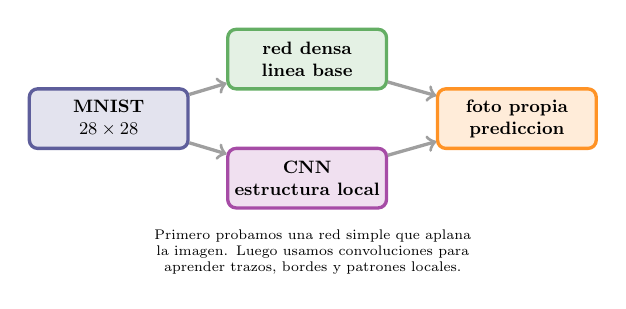
\begin{tikzpicture}[scale=0.72,transform shape]
\tikzstyle{box}=[draw,rounded corners=3pt,very thick,minimum width=2.8cm,minimum height=1.05cm,align=center,font=\small\bfseries]
\node[box,fill=MidnightBlue!12,draw=MidnightBlue!70] (mnist) at (0,0) {MNIST\\$28\times28$};
\node[box,fill=ForestGreen!12,draw=ForestGreen!70] (dense) at (3.5,1.05) {red densa\\linea base};
\node[box,fill=Purple!12,draw=Purple!70] (cnn) at (3.5,-1.05) {CNN\\estructura local};
\node[box,fill=orange!15,draw=orange!85] (photo) at (7.2,0) {foto propia\\prediccion};
\draw[->,very thick,gray!75] (mnist) -- (dense);
\draw[->,very thick,gray!75] (mnist) -- (cnn);
\draw[->,very thick,gray!75] (dense) -- (photo);
\draw[->,very thick,gray!75] (cnn) -- (photo);
\node[font=\scriptsize,align=center,text width=8.2cm] at (3.6,-2.35) {Primero probamos una red simple que aplana la imagen. Luego usamos convoluciones para aprender trazos, bordes y patrones locales.};
\end{tikzpicture}
